%% This is an example first chapter.  You should put chapter/appendix that you
%% write into a separate file, and add a line \include{yourfilename} to
%% main.tex, where `yourfilename.tex' is the name of the chapter/appendix file.
%% You can process specific files by typing their names in at the 
%% \files=
%% prompt when you run the file main.tex through LaTeX.
\chapter{Computing orders of component groups and Tamagawa numbers of Jacobians}\label{papertwo}

\section{Explicit computation of the orders of component groups}\label{compgroup}
\subsection{The weighted dual graph}\label{weightdualgraph}
Let $C$ be a nice $K$-curve and let $X$ be a proper regular model of the curve $C$ over $R$. The {\color{blue}{\textsf{weighted dual graph}}} $G$ of $X_s$ is defined as follows. The vertices of $G$ are the irreducible components of $X_s$. For each vertex $v$ of $G$, let $\Gamma_v$ denote the corresponding irreducible component of $X_s$ and let $m_v$ denote the multiplicity of $\Gamma_v$ in $X_s$. The number of edges between two distinct vertices $v$ and $w$ equals $\Gamma_v.\Gamma_w$. There are no edges connecting a vertex to itself. For every edge $e$ between the vertices $v$ and $w$, the  weight of $e$, denoted $\wt(e)$, is defined to be $m_v m_w$. 

\begin{rmk}
 This is the graph obtained by deleting all the loops (i.e., the edges that connect a vertex to itself) in the usual dual graph associated to $X_s$ that is used in algebraic geometry. Including the loops will not alter the proof below, since a graph and the associated loopless graph have the same Laplacian operator.
\end{rmk}

Let $\Phi$ denote the component group scheme of the N\'{e}ron model of the Jacobian of $C$. 

\begin{rmk}
 Let $\beta$ be the map defined in Theorem~\ref{mainthmblr}. The component group associated to the pair $(G,\beta)$ (as defined in Section~\ref{intrograph}) coincides with $\Phi(\overline{k})$. In fact, the map $\alpha$ in Section~\ref{intrograph} coincides with the map $\alpha$ in Theorem~\ref{mainthmblr}.
\end{rmk}

In this section, we give a formula for $\Phi(\overline{k})$ in terms of the graph $G$. Special cases of this formula already appear in \cite{lor2}; see, for instance, Proposition $4.19$ therein. A version of this formula is also implicit in the proof of \cite[Corollary~3.5]{lor1}. 

\subsection{The formula}\label{raynaudsformula}

\begin{thm}\label{compformula}
Let $m = \gcd(m_v \ | \ v \in V(G))$. Let $\Phi$ denote the component group scheme of the N\'{e}ron model of the Jacobian of $C$. Then
 \begin{equation}\label{formula}
  \# \Phi(\overline{k}) = m^2 \left( \sum_{T \in S(G)} \prod_{v \in V(T)} m_{v}^{\# N_T(v)-2} \right) . 
 \end{equation} 
\end{thm}
\begin{proof}
Let $r = \# V(G)$. As in the statement of Corollary~\ref{maincorblr}, let $M$ be the $r \times r$ matrix corresponding to the intersection pairing. Let $a_v$ denote the absolute value of the $(r-1) \times (r-1)$ minor that we get from $M$ by deleting the row and column corresponding to the vertex $v$. Corollary~\ref{maincorblr} shows that if $v \in V(G)$, then the order of the component group is equal to $(\tfrac{m}{m_v})^2 a_v$. Let $(N_{vv'})$ be the $r \times r$ matrix defined by $N_{vv'} = m_v m_{v'} M_{vv'}$ for every $v,v' \in V(G)$. Fix a vertex $\tilde{v}$ of $G$. Let $b$ denote the absolute value of the $(r-1) \times (r-1)$ minor that we get from $N$ by deleting the row and column corresponding to the vertex $\tilde{v}$. Then
\begin{align*}
 \# \Phi(\overline{k}) &= \left( \frac{m}{m_{\tilde{v}}} \right)^2 a_{\tilde{v}} \\
 &= \frac{m^2}{(\prod_{v \in V(G)} m_{v})^2} b \\
 &=  \frac{m^2}{(\prod_{v \in V(G)} m_{v})^2}  \sum_{T \in S(G)} \prod_{e \in E(T)} \wt(e) \ \ \ \ (\textup{by Theorem}~\ref{matrixtreeforgraphs}) \\ 
 &=  \frac{m^2}{(\prod_{v \in V(G)} m_{v})^2}  \sum_{T \in S(G)} \prod_{v \in V(T)} m_{v}^{\# N_T(v)} \\
 &=  m^2 \left( \sum_{T \in S(G)} \prod_{v \in V(T)} m_{v}^{\# N_T(v)-2} \right), 
\end{align*}
since $V(T) = V(G)$ for any spanning tree $T$ of $G$.
\end{proof}

\begin{rmk}
 The formula also holds under the assumption that $R$ is merely strictly henselian, provided we also assume that all the $e_i$ are equal to $1$ and that $X$ admits a section.
\end{rmk}
\begin{rmk}
 If the dual graph $G$ is a tree, the formula simplifies to 
 \[ \# \Phi(\overline{k}) = m^2 \prod_{v \in V(G)} m_{v}^{\# N_G(v)-2} .\] 
\end{rmk}
\begin{rmk}
 Specializing to the case where $C$ is an elliptic curve, we recover the correct orders of the component groups for each of the Kodaira types. 
\end{rmk}

\subsection{Applications of the formula}
\subsubsection{Criterion for uniform bounds on the orders of component groups}
In the case of elliptic curves, the order of the component group is bounded above by $4$ if we exclude curves of reduction type $I_n$. In the theorem below, we provide a generalization of this fact for higher genus curves. We begin by proving a lemma in graph theory.

\begin{lemma}\label{graph}
 A vertex $v$ of a graph $G$ belongs to some cycle of $G$ if and only if there exists a spanning tree $T$ of $G$ and an edge $e \in E(G)$ such that $v \in D(e)$ and $e \notin E(T)$.
\end{lemma}
\begin{proof}[Sketch of proof]
The `if' direction follows from the fact that adding any edge of $E(G) \setminus E(T)$ to a spanning tree produces a graph that contains a cycle. The `only if' direction follows from the fact that any spanning tree of $(V(G),E(G)\setminus \{e\},w)$ is a spanning tree of $G$, where $e$ is an edge in a cycle having $v$ as an endpoint.
\end{proof}

\begin{thm}\label{uniformbound}
 Assume that $X/S$ is the minimal proper regular model of the curve $C/K$ and that the genus $g$ of $C$ satisfies $g \geq 2$. Let $G$ be the dual graph of $X_s$. Assume further that if $v \in V(G)$ corresponds to a $(-2)$-curve (that is, a $\P^1_k$ of self-intersection $-2$), then $v$ does not belong to any cycle of $G$. Then there exists an integer $n(g)$, depending only on the genus $g$ of $C$, such that the order of the component group of the special fiber of the N\'{e}ron model of the Jacobian of $C$ is bounded above by $n(g)$.
\end{thm}
\begin{proof}
Lemma~\ref{graph} and the assumption on $(-2)$-curves in the theorem imply that the edges in any chain of $(-2)$-curves belong to every spanning tree. In other words, every chain of $(-2)$-curves is a connecting chain. Contracting all chains of $(-2)$-curves produces a graph $G'$. \cite[Corollary~4.3]{winters} implies that $G'$ is the dual graph of the special fiber of a regular $S$-curve $X'$. Since a vertex $v$ that is part of a connecting chain has exactly two neighbours in every spanning tree, the exponent $N_T(v)-2$ equals $0$ for every spanning tree $T$ for every such vertex. It follows that such a vertex does not contribute to the order of the component group by formula~\eqref{formula}. This implies that the order of the component group of $G'$ equals the order of the component group of $G$. Since we also assumed that $X$ is minimal and $g \geq 2$, Theorem~\ref{finsim} implies that there are only finitely many possibilities for the weighted dual graph of $X_s'$, if we fix the genus $g$ of $X'_{\eta}$. For a fixed $g$, we can compute the order of the component group of the special fiber of the N\'{e}ron model of the Jacobian for each of these finitely many weighted dual graphs and take the maximum of these numbers to be $n(g)$. 
\end{proof}

\begin{rmk}
 The condition in the theorem above is strictly weaker than requiring the toric rank of $C$ be $0$. The toric rank $0$ condition would imply that the graph $G$ has no cycles.
\end{rmk}

\begin{rmk}
 A na\"{i}ve bound for $n(g)$ that one gets by examining the Artin--Winters argument is $n(g) \sim O((2g-2)^{8(2g-2)^2})$. It might be possible to improve this bound by analyzing the combinatorics of these graphs more carefully.
\end{rmk}

\subsubsection{Structure of the component group: periodicity}
We will now prove an analogue of \cite[Corollary~4.7]{bano}. The key step in the proof of Theorem~\ref{uniformbound} is the fact that contracting connecting chains in the dual graph does not alter the order of the component group. The structure of the group, however, does depend on the length of the chain. For example, the Kodaira types $I_n^*$ all have component groups of order $4$, but the component group is either $\Z/2\Z \times \Z/2\Z$  or $\Z/4\Z$ depending on whether $n$ is even or odd. In this example, the structure of the component group only depends on the length of the connecting chain modulo $2$. This suggests that if we have a family of dual graphs which only differ in the length of a single connecting chain, and if all the vertices in the connecting chain have multiplicity $m$, then the structure of the component group should be $m$-periodic, i.e., it should depend only on the length of the chain modulo $m$. More precisely:

\begin{thm}\label{compcontract}
 Let $(G,\beta)$ be a graph equipped with a multiplicity function. Let $L$ be a length $m$ connecting chain in $G$ such that $\beta(v) = m$ for all $v \in V(L)$. Define $\alpha$ as in Section~\ref{intrograph}. Assume that $\alpha_{v,v} = -2$ for every $v \in V(L)$. Let $(G',\beta')$ be the pair obtained by contracting the chain $L$. Then the component group of $(G',\beta')$ is isomorphic to the component group of $(G,\beta)$.
\end{thm}
\begin{proof}
\begin{figure}[H]
 \centering
 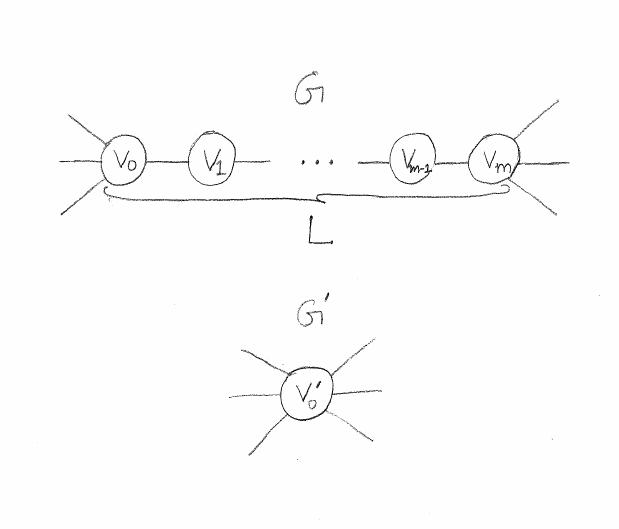
\includegraphics[scale=0.6]{contraction}
\end{figure}
Let $\Phi(G) = \ker \beta/\im \alpha$ and let $\Phi(G') = \ker \beta'/\im \alpha'$ as in Section~\ref{intrograph}. Choose an ordering $(v_0,v_1,\ldots,v_m)$ of $V(L)$ as in the definition of a chain, and let $\{v_0'\}$ be the image of $V(L)$ in $V(G')$. Let $f_0 \colon V(G') \rightarrow V(G)$ be the section of the natural quotient map $V(G) \rightarrow V(G')$ that satisfies $f_0(v_0') = v_0$. Let $f \colon \Z^{V(G')} \rightarrow \Z^{V(G)}$ be the linear map defined by $f_0$ on the corresponding basis elements. We will now define another map $h$ such that the maps in the following diagram commute. 
 \begin{equation*}
 {\xymatrix{
\Z^{V(G')} \ar[dd]_{h} \ar[rr]^{\alpha'} & & \Z^{V(G')} \ar[dd]_{f} \ar[rr]^{\beta'} & & \Z \ar@{=}[dd] \\
& & & & \\
\Z^{V(G)} \ar[rr]^{\alpha} & & \Z^{V(G)} \ar[rr]^{\beta} & & \Z. 
}}
\end{equation*} 
Then $f$ will induce a homomorphism from the homology $\Phi(G')$ of the top row to the homology $\Phi(G)$ of the bottom row. 

We will describe $h$ by giving its value on each $v' \in V(G')$. In order to define $h$, for every $v' \in V(G')$, it suffices to find $v \in \Z^{V(G)}$ (depending on $v'$) such that $\alpha (v) = f(\alpha'(v'))$; we can then define $h(v') = v$. 

{\bf{Case 1:}} $v' \notin \{v_0'\} \cup f_0^{-1}(N_G(v_m))$. \\
In this case, let $h(v') \colonequals f_0(v')$. Since the edges emanating from $v'$ are in bijection with the edges emanating from $f_0(v')$, it follows that $\alpha (f_0(v')) = f(\alpha' (v'))$. 

{\bf{Case 2:}} $v' \in f_0^{-1}(N_G(v_m)) \setminus \{v_0'\}$. \\
In this case $f(\alpha'(v')) = \alpha(f_0(v'))+\Gamma_{v'}.\Gamma_{v_0'}(v_m-v_0)$. It therefore suffices to find $t_1 \in \Z^{V(G)}$ such that $\alpha(t_1) = \Gamma_{v'}.\Gamma_{v_0'}(v_m-v_0)$, since we can then define $h(v') = f_0(v')+t_1$. 

Let $V(G) \setminus V(L) = D_0 \cup D_m$, where $D_0$ (respectively $D_m$) consists of the vertices of $G$ having a path to $L$ meeting $L$ only at $v_0$ (respectively $v_m$). Let $t = mv_m+\sum_{w \in D_m} \beta(w) w$. If $v \notin D_m \cup \{v_{m-1},v_m\}$, then the vertex $v$ has no neighbours in $D_m \cup \{v_m\}$, so the coefficient of $v$ in $\alpha(t)$ is $0$. For any vertex $v$, we have $\alpha(v) = \alpha_{v,v} v + \sum_{w \in N_G(v)} \alpha_{v,w} w$; it follows that if $v \in D_m$, then the coefficient of $v$ in $\alpha(t)$ equals the coefficient of $v$ in $\alpha(\sum_{w \in V(G)} \beta(w) w)$. The latter is $0$ since $\sum_{w \in V(G)} \beta(w) \alpha_{w',w} = 0$ for every $w' \in V(G)$.  By a similar argument, the coefficient of $v_m$ in $\alpha(t+\beta(v_{m-1})v_{m-1})$ is $0$ since it equals the coefficient of $v_m$ in $\alpha(\sum_{w \in V(G)} \beta(w) w)$. The same type of argument also shows that the coefficient of $v_{m-1}$ in $\alpha(t-mv_m)$ is $0$. Since $\beta(v_{m-1}) = \beta(v_m) = m$, we conclude that $\alpha(t) = mv_{m-1}-mv_m$. 

Fix $j$ such that $0 \leq j \leq m-1$. Let $x_j = \sum_{i=1}^j iv_i$. Since $\alpha(v_j) = v_{j-1}-2v_j+v_{j+1}$, an inductive argument shows that $\alpha(x_j) = v_0-(j+1)v_j+jv_{j+1}$. Let $t_1 = -\Gamma_{v'}.\Gamma_{v_0'}(x_{m-1}+t)$. It follows that $\alpha(t_1) = \Gamma_{v'}.\Gamma_{v_0'}(v_m-v_0)$.

{\bf{Case 3:}} $v' = v_0'$. \\
We have $f(\alpha'(v_0')) = \alpha(v_0+v_m)-v_1-v_{m-1}+2v_m$. It therefore suffices to find $t_2 \in \Z^{V(G)}$ such that $\alpha(t_2) = 2v_m-v_1-v_{m-1}$. We may then define $h(v_0') = v_0+v_m+t_2$. 
 
Let $t$ be defined as in Case 2. For $1 \leq j \leq m-1$, let $y_j = \sum_{i=1}^j (i-1)v_i$. Once again an inductive argument as in Case 2 shows that $\alpha(y_j) = v_1-jv_j+(j-1)v_{j+1}$. Let $t_2 = -y_{m-1}-t$. Then $\alpha(t_2) = 2v_m-v_1-v_{m-1}$.

We have now proved that $f$ induces a well-defined map from $\Phi(G')$ to $\Phi(G)$. We want to prove that this map is an isomorphism. Since $|\Phi(G')| = |\Phi(G)|$ (by the proof of Theorem~\ref{uniformbound}), it suffices to prove that it is a surjection. Let $u \in \ker \beta$. We will inductively construct a sequence of elements $u_0,u_1,\ldots,u_m$ such that 
 \begin{itemize}
  \item $u_0 = u$ and $u_m \in \im f$,
  \item For every $i$ satisfying $0 \leq i \leq m-1$, we have $u_{i+1}-u_i \in \im \alpha \subset \ker \beta$. 
  \item For every $i$ satisfying $1 \leq i \leq m$, and for every $j \in \{{m-i+1},{m-i+2},\ldots,m\}$, the coefficient of $v_j$ in $u_i$ is $0$.  
 \end{itemize}
 For the inductive step, suppose that $1 \leq i \leq m-2$ and $u_i = \sum -a_v v$, where $a_v \in \Z$. Let 
 \[ u_{i+1} = u_i + \alpha(a_{v_{m-i}} v_{m-i-1}) = u_i+a_{v_{m-i}}(v_{m-i-2}-2v_{m-i-1}+v_{m-i}) .\] 
 From the equation above, it follows that for $j \in \{m-i+1,m-i+2,\ldots,m \}$ the coefficient of $v_j$ in $u_{i+1}$ is the same as that in $u_i$, and that the coefficient of $v_{m-i}$ in $u_{i+1}$ is $-a_{v_{m-i}}+a_{v_{m-i}} = 0$. The induction hypothesis implies that $a_{v_j} = 0$ for $j \in \{m-i+1,m-i+2,\ldots,m\}$. This finishes the induction. So to finish the construction, it now suffices to prove that $u_m \in \im f$. 
 
 Let $T = V(G) \setminus \{v_1,v_2,\ldots,v_m\}$. By the definition of the map $f$, it maps $\Z^{V(G')}$ isomorphically on to the subset of elements of $\Z^{V(G)}$ supported on $T$. This isomorphism maps $\ker \beta'$ isomorphically to the set of elements of $\ker \beta$ supported on $T$. Since $u_m \in \ker \beta$ and is supported on $T$, this shows that $u_m \in \im f$.  Since $u_m-u_0 \in \im \alpha$, this completes the proof of surjectivity of $f$ on to $\Phi(G)$.   
\end{proof}

\begin{rmk}
 Fix $g$. If $\cha k = 0$, then it is possible to list all the groups that can arise as the component group of the Jacobian of a nice curve of genus $g$ by combining the theorem above with Theorem~\ref{finsim} and Theorem~\ref{typeexistence}.
\end{rmk}

\subsubsection{The N\'{e}ron component series for Jacobians}\label{altprfcomp}
In this section, we provide an alternate proof of \cite[Chapter~3, Proposition~3.1.1]{halnic}, that works in both the equal characteristic and mixed characteristic cases. For the proof, we use the explicit formula in Theorem~\ref{compformula} and the behaviour of {\textup{snc}} models under tame extensions, as described in Section~\ref{deftameext}.

\begin{prop}\cite[Chapter~3, Proposition~3.1.1]{halnic}\label{newproof}
 Let $X$ be the minimal {\textup{snc}} model of a nice $K$-curve of genus $g \geq 1$. Let $d \in \N'$ be an integer prime to $e(X)$. Let $\mathcal{A}$ denote the N\'{e}ron model of the Jacobian of $X_\eta$ and let $\mathcal{A}(d)$ denote the N\'{e}ron model of the Jacobian of $X \times_K K(d)$. Let $t$ denote the toric rank of $\mathcal{A}$. Then
 \[ |\Phi(\mathcal{A}(d))| = d^t |\Phi(\mathcal{A})| .\]
\end{prop}
\begin{proof}
 Let $X(d)$ be the minimal desingularization of the normalization $X_d$ of $X \times_R R(d)$. Let $G$ be the dual graph of $X_s$ and let $G'$ be the dual graph of $X(d)_s$. As mentioned before Proposition~\ref{comodel}, $X(d)$ is a {\textup{snc}} model. Let $J$ be the Jacobian of $X_\eta$.
  
 {\bf{Case 1:}} $J$ is an elliptic curve with multiplicative reduction.\\
  In this case, \cite[Theorem~6.6]{llr} tells us that the minimal {\textup{snc}} model and the minimal regular model coincide, and $X_s$ is also a cycle of rational curves, where the rational curves in the cycle all have the same multiplicity, say $m$. Since the number of spanning trees of $G$ equals the number of vertices in the cycle, and for each spanning tree $T$, the product $\prod_{v \in V(T)} m_v^{N_T(v)-2}$ equals $1/m^2$, the explicit formula in Theorem~\ref{compformula} implies that the order of the component group of the N\'{e}ron model of $J$ equals the number of vertices in the cycle $G$.   
  
  We will first show that $X(d)_s$ is also a cycle of rational curves, and then compute the number of rational curves in the cycle. Formula~\ref{formula} would once again imply that the order of the component group equals the number of vertices in the cycle $G'$.
 
 Proposition~\ref{comodel}(ii) implies that every component of $(X_d)_s$  intersects exactly two other components. Since $(X_d)_s$ is connected by Zariski's connectedness principle, we conclude that it is a cycle of rational curves. Proposition~\ref{comodel}(iii) tells us that in order to obtain $X(d)_s$ from $(X_d)_s$, we have to replace each node in the cycle of rational curves by a chain of rational curves of appropriate length. This implies that $(X_d)_s$ is also a cycle of rational curves. Now,
 \begin{itemize}
  \item Proposition~\ref{comodel}(ii) implies that the number of irreducible components of $(X_d)_s$ equals $\gcd(d,m)$ times the number of irreducible components of $X_s$. 
  \item Proposition\ref{comodel}(iii) and Proposition~\ref{combdata} imply that the preimage of each singular point of $(X_d)_s$ is a chain of rational curves, where the number of rational curves in the chain equals $d/\gcd(d,m)$. 
  \item The number of singular points of $(X_d)_s$ equals the number of irreducible components of $(X_d)_s$. 
 \end{itemize}
 Combining the arguments above, we conclude that the number of irreducible components of $X(d)_s$ is $d$ times the number of irreducible components of $X_s$, and this finishes the proof in this case, since the toric rank $t$ equals $1$.
 
 {\bf{Case 2:}} $J$ is not an elliptic curve with multiplicative reduction. \\
 Then either $g \geq 2$, or $J$ is an elliptic curve with good or additive reduction. Lemma~\ref{dgraphbaseext} implies that $X_s$ and $(X_d)_s$ have the same dual graph. Proposition~\ref{comodel}(iii) implies that $G'$ is a subdivision of $G$. Let $\pi \colon E(G') \rightarrow E(G)$ be the surjective map that maps an edge of $G'$ to the unique edge in $G$ that it is a subdivision of. Let $v$ and $w$ be neighbouring vertices of $G$. In this case, the proof of \cite[Lemma~2.3.2]{halnic} tells us that $\gcd(d,m_v,m_w) = 1$. Let
 \begin{itemize}
  \item $h_v = \gcd(d, m_v)$, 
  \item $h_w = \gcd(d, m_w)$,
  \item $m_v = h_v m_v'$,
  \item $m_w = h_w m_w'$, and,
  \item $d = h_v h_w d'$.
 \end{itemize}
 Then $dm_v' m_w' = d'm_v m_w$. Let $v'$ and $w'$ be the corresponding vertices of $G'$ and let $u_1, u_2, \ldots, u_\lambda$ be the intermediate vertices. Then Lemma~\ref{dgraphbaseext}(ii) tells us that $m_{v'} = m_v'$ and $m_{w'} = m_w'$. Let $r$ be the unique solution to $rm_{v'}+m_{w'} = 0 \mod d'$. Let $(\mu_1,\mu_2, \ldots, \mu_{\lambda})$ be the multiplicity vector associated to the tuple $(d',r,m_{v'},m_{w'})$. By Proposition~\ref{combdata} $m_{u_i} = \mu_i$. By Lemma~\ref{curious},
 \begin{equation}\label{scale}
 \frac{d}{m_v m_w} = \frac{d'}{m_v' m_w'} = \frac{1}{m_v' \mu_1} + \frac{1}{\mu_1 \mu_2} + \cdots + \frac{1}{\mu_{\lambda-1} \mu_\lambda} + \frac{1}{\mu_\lambda m_w'} . 
 \end{equation}
 
 Let $H$ be a connected graph. Let $S(H)$ be the collection of spanning trees of $H$. The first Betti number $t(H)$ of a connected graph $H$ equals $|V(H)|-|E(H)|+1$. Let $T \in S(H)$. Since $|V(H)| = |V(T)|$, and the first Betti number of a tree equals $2$, it follows that $\# (E(H) \setminus E(T)) = t(H)$. For a spanning tree $T$ of a dual graph $H$, let $\phi(T) = \prod_{v \in V(H)} m_v^{N_T(v)-2}$. Fix a dual graph $H$. Let $\delta \colon E(H) \rightarrow \N$ be the map defined by $\delta(e) \colonequals m_v m_w$, where $v$ and $w$ are the endpoints of $e$, and $m_v$ and $m_w$ are the multiplicities of the corresponding irreducible components in the special fiber. 
 
 Fix $T' \in S(G')$. Let $T$ be the subgraph of $G$ such that $V(T) = V(G)$ and such that $E(T) = \{ e \in E(T) \ | \ \pi^{-1}(e) \subset E(T') \}$. Since $G'$ is a subdivision of $G$, it follows that $T$ is a spanning tree of $G$. The construction $T' \mapsto T$ defines a map $\tau \colon S(G') \rightarrow S(G)$. Let $T' \in S(B')$ and let $\tau(T') = T$. Let $B' = E(G') \setminus E(T')$ and let  $B = E(G) \setminus E(T)$. Let $\pi_T$ be the restriction of $\pi$ to $\pi^{-1}(B)$. Let $\epsilon \colon \pi^{-1}(B) \rightarrow \Q^\times$ be the map defined by $\epsilon(e) = \delta(\pi(e))/\delta(e)$. Since $G'$ is a subdivision of $G$, it follows that
 \begin{itemize}
  \item $t(G') = t(G)$, and,
  \item there is a multiplicity-preserving bijection between the vertices of $T'$ of degree $\geq 3$ and those of $T$ of degree $\geq 3$.
 \end{itemize}
The two facts above imply that 
\[ \phi(T')/\phi(T) = \prod_{e \in B'} \epsilon(e) .\]
Since $G'$ is a subdivision of $G$, it follows that there exists a bijection
\[ \{ T'' \in S(G') \ | \ \tau(T'') = T \} \longleftrightarrow \textup{Sections } \sigma \colon B \rightarrow \pi^{-1}(B) \textup{ of } \pi_T .\]
Let $\mathfrak{s}$ denote the set of sections of $\pi_T$. Since $t(G) = t(G')$, and the toric rank $t$ equals the first Betti number of the graphs $G$ and $G'$ (by \cite[9.2.5,9.2.8]{blr}), it follows that $\# B = \# B' = t$. Now
\begin{align*} \sum_{T' \in \tau^{-1}(T)} \frac{\phi(T')}{\phi(T)} &= \sum_{\sigma \in \mathfrak{s}} \prod_{e \in B} \epsilon (\sigma(e)) \\
&= \prod_{e \in B} \sum_{e' \in \pi^{-1}(e)} \epsilon(e') \\
&= \prod_{e \in B} \delta(e) \sum_{e' \in \pi^{-1}(e)} \frac{1}{\delta(e')} \\
&= \prod_{e \in B} \delta(e) \frac{d}{\delta(e)} \ \ \ (\textup{by Equation~\eqref{scale}}) \\
&= d^{\# B} = d^t.
\end{align*}
Now
\[ \sum_{T' \in S(G')} \phi(T') = \sum_{T \in S(G)} \sum_{T' \in \tau^{-1}(T)} \phi(T') = d^t \sum_{T \in S(G)} \phi(T)  .\]
To finish the proof, it suffices to prove that $\gcd(m_v \ | \ v \in V(G)) = \gcd(m_{v'} \ | \ v' \in V(G'))$ by the formula in Theorem~\ref{compformula}. Lemma~\ref{gcdmult} implies that the gcd of the multiplicities of the components of $X_d$ and the gcd of the multiplicities of the components of $X(d)$ are equal. This implies that it now suffices to prove $\gcd(m_v \ | \ v \in V(G)) = \gcd(m_v/\gcd(m_v,d) \ | \ v \in V(G))$. The right hand side divides the left hand side. To prove the other divisibility, we use the fact that $G$ is connected, and the fact that if $v$ and $w$ are any pair of neighbouring vertices in $G$, then $\gcd(m_v,m_w,d) = 1$ (this follows from the proof of Lemma~\ref{dgraphbaseext} in \cite{halnic}). This concludes the proof. \qedhere
\end{proof}

\section{Explicit computation of Tamagawa numbers}\label{tamagawa}
%Let $C$ be a nice curve over $K$ and let $X$ be a regular model for $C$ over $R$. The component group $\Phi$ which was defined in Section~\ref{compgroup} is in fact the set of $\overline{k}$ points of a finite \'{e}tale $k$-group scheme $\phi$, called the component group scheme. The order of the set of $k$ points of this scheme is the Tamagawa number associated to the curve $C$. 

In this section, we will show that we can use a version of the matrix-tree theorem for directed weighted multigraphs to compute Tamagawa numbers. The notation used in this section is consistent with the notation in Section~\ref{introtam}. 

% In this section, we do not assume that the residue field $k$ is algebraically closed. We assume that $k$ is perfect and we let $\overline{k}$ denote an algebraic closure of $k$. Let $R^{\textup{st}}$ denote the strict henselization of $R$. Let $X$ be a regular $S$-curve. 

\subsection{The quotient graph $\widetilde{G}$}
Let $X^{\textup{st}} = X \times_R R^{\textup{st}}$. Let $G$ denote the dual graph of $X^{\textup{st}}_s$, and let $V = V(G)$. We now define a directed weighted multigraph $\widetilde{G}$, which we call the quotient graph. The set of vertices of $\widetilde{G}$, which we denote $\widetilde{V}$, is the the set of irreducible components of $X_s$. The set $\widetilde{V}$ can also naturally be identified with the set of orbits of $V$ under the natural action of $\Gal (\overline{k}/k)$. This identification gives rise to a quotient map $\pi \colon V \rightarrow \widetilde{V}$ where we map a vertex $v$ to the corresponding orbit. For any two vertices $\tilde{w}$ and $\tilde{v}$ in $\widetilde{V}$, the number of directed edges with tail $\tilde{w}$ and head $\tilde{v}$, which we denote $\alpha_{\tilde{w} \tilde{v}}$, is defined as follows. Fix any $w \in \pi^{-1}(\tilde{w})$.  Then $\alpha_{\tilde{w} \tilde{v}} = \sum_{v \in \pi^{-1}(\tilde{v})} \Gamma_v.\Gamma_w$. Since the Galois action transitively permutes the 
vertices $w \in \pi^{-1}(\tilde{w})$ and preserves intersection numbers, the sum is independent of the choice of $w \in \pi^{-1}(\tilde{w})$. This defines the vertices and directed edges of $\widetilde{G}$.

We now define a weight function on $\widetilde{G}$. For every $\tilde{v} \in \widetilde{V}$, let $|\tilde{v}|$ denote the size of the orbit corresponding to $\tilde{v}$. For any $\tilde{v} \in \widetilde{V}$, let $\Gamma_{\tilde{v}}$ denote the corresponding irreducible component of $X_s$, and let $m_{\tilde{v}}$ denote the multiplicity of $\Gamma_{\tilde{v}}$ in the special fiber $X_s$. For any directed edge $e$ with tail $\tilde{w}$ and head $\tilde{v}$, the weight of the edge $e$, denoted $\wt(e)$ is defined to be $m_{\tilde{v}} m_{\tilde{w}} |\tilde{w}|$. 

\subsection{Explicit computation of Tamagawa numbers}
In this section, we will show how to combine Theorem~\ref{galcoh} and Theorem~\ref{matrixtree} to explicitly compute Tamagawa numbers. In the rest of this section, we will assume that $\Gal (\overline{k}/k)$ is procyclic in order to be able to apply Theorem~\ref{galcoh}.

\begin{rmk}
The order of the component group can also be computed using using Theorem~\ref{matrixtree} (this corresponds to the special case where $k = \overline{k}$). The formula that we obtain for the component group using Theorem~\ref{matrixtree} can be checked to be equal to the formula obtained in Theorem~\ref{compformula}. We included the proof in Section~\ref{compgroup} since the graph that appears in Section~\ref{compgroup} is more closely related to the dual graph that appears in algebraic geometry.
\end{rmk}

Let $\alpha$ and $\beta$ be as in Section~\ref{introtam}. We now show that if we make the appropriate modifications to $\alpha$ and $\beta$, we can use Theorem~\ref{matrixtree} to compute Tamagawa numbers. Define maps $\delta_1, \delta_2, \alpha_1,\beta_1,\beta_2$ as follows:
\begin{align*}
 \delta_1 \colon \Z^{\widetilde{V}} &\rightarrow \Z^{\widetilde{V}} \\
 (b_{\tilde{v}}) &\mapsto (b_{\tilde{v}}m_{\tilde{v}}|\tilde{v}|) \\
 \delta_2 \colon \Z^{\widetilde{V}} &\rightarrow \Z^{\widetilde{V}} \\
 (b_{\tilde{v}}) &\mapsto (b_{\tilde{v}}m_{\tilde{v}}) \\
\alpha_1 = \delta_1 &\circ \alpha \circ \delta_2 \\
\beta_1 \colon \Z^{\widetilde{V}} &\rightarrow \Z \\
 (b_{\tilde{v}}) &\mapsto \sum_{\tilde{v} \in \widetilde{V}} b_{\tilde{v}} \\
\beta_2 \colon \Z &\rightarrow \Z^{\widetilde{V}} \\
 b &\mapsto (b,b,\ldots,b)  .
\end{align*}
We have $\beta_1 \delta_1 = \beta$, so $\beta_1 \alpha_1 = \beta_1 \delta_1 \alpha \delta_2 = \beta \alpha \delta_2 = 0$. This implies that $\im(\alpha_1) \subset \ker{\beta_1}$.

We now prove a lemma in linear algebra that allows us to compare the orders of the finite groups $\ker(\beta_1)/\im(\alpha_1)$ and $\ker(\beta)/\im(\alpha)$.
\begin{lemma}\label{linear}
Let $n$ be a nonnegative integer. Let $D, D' \colon \Z^n \rightarrow \Z^n$ be two rank $n$ linear operators whose matrices are diagonal. Let $A \colon \Z^n \rightarrow \Z^n$ be a rank $n-1$ linear operator. Let $S \colon \Z^n \rightarrow \Z$ denote the linear operator which takes a vector to the sum of its coordinates, and let $\Delta \colon \Z \rightarrow \Z^n$ denote the diagonal embedding. Assume $SDA = 0$ and $AD'\Delta = 0$. Let $d,d'$ be positive integers such that $d\Z = \im \left( SD \right)$ and $d'\Z = \im \left( SD' \right)$ respectively. Then
\begin{equation}\label{lalg} \# \frac{\ker (S D) }{\im A} = \frac{d}{|\det D|} \cdot \# \frac{\ker S }{\im (D A)} = \frac{dd'}{|\det D| |\det D'|} \cdot \# \frac{\ker S }{\im ( D A D' )} .\end{equation}
\end{lemma}
\begin{proof}
 The integer $d$ is the gcd of the diagonal entries of $D$. Thus $\tfrac{1}{d} D \in M_n(\Z)$. Similarly $\tfrac{1}{d'} D' \in M_n(\Z)$. Replacing $D$ by $\tfrac{1}{d}D$ and replacing $D'$ by $\tfrac{1}{d'}D'$ multiplies the five ratios in Equation~\eqref{lalg} by $1,d^{n-1},d^{1-n},(dd')^{n-1}$ and $(dd')^{1-n}$ respectively. Therefore we may assume $d=d'=1$ without any loss of generality.
 
We now prove the first equality. For this, we show that the following sequence is exact.
\[ 0 \rightarrow \frac{\ker (SD)}{\im A} \xrightarrow{D} \frac{\ker S}{\im (DA)} \rightarrow \frac{\Z^n}{\im D}  \rightarrow 0 . \]
The exactness at the left follows because $D$ is an injection, and therefore restricts to an injection from $\ker (SD)$ to $\ker S$, and also implies that $D^{-1} (\im (DA)) = \im A$. The exactness at the middle follows because $D(\ker (SD)) = \ker S \cap \im D$. For the exactness on the right, it suffices to show that $\Z^n/(\ker S + \im D) = 0$. This follows because $\Z^n/(\ker S + \im D) \simeq \im S/\im(SD) = \Z/d\Z = 0$, since $d=1$. Since all the groups in the above exact sequence are finite and $\# \left( \tfrac{\Z^n}{\im D} \right) = |\det D|$, we get 
\[ \# \frac{\ker (S D) }{\im A} |\det D| =  \# \frac{\ker S }{\im (D A)} .\]
This finishes the proof of the first equality.

Let $A' = DA$. For the second equality, we show that the following sequence is exact.
\[ 0 \rightarrow \frac{\Z^n}{\im D'} \xrightarrow{A'} \frac{\ker S}{\im (A'D')} \rightarrow \frac{\ker S}{\im A'} \rightarrow 0  .\]
First, since $SA' = SDA = 0$, the map on the left is well-defined. Since $d'=1$, it follows that $\im D'\Delta$ is a rank $1$ lattice generated by a primitive vector, and therefore is a saturated submodule of $\Z^n$. On the other hand, we have $\im D' \Delta \subset \ker A'$ (since $A'D'\Delta = DAD'\Delta = 0$), and $\ker A'$ is also a rank $1$ lattice (since $D'$ is injective and $A$ has rank $n-1$). Therefore we must have $\im D' \Delta = \ker A'$, which implies that $\ker A' \subset \im D'$. This in turn implies that $A'^{-1}(\im A'D') = \im D' + \ker A' = \im D'$. This proves exactness on the left of the sequence above. The exactness at the other two positions is immediate.
\end{proof}

\begin{lemma}\label{compare}
Let $m$ and $\tilde{m}$ be as defined as in Theorem~\ref{galcoh}. 
\[ \# \left( \frac{\ker{\beta}}{\im{\alpha}} \right)  = \frac{m \tilde{m}}{\prod_{\tilde{v} \in \widetilde{V}} m_{\tilde{v}}^2 |\tilde{v}| } \ \# \left( \frac{\ker{\beta_1}}{\im{\alpha_1}} \right) .\] 
\end{lemma}
\begin{proof}
This follows directly from Lemma~\ref{linear} with $A = \alpha, D = \delta_1$ and $D' = \delta_2$. \qedhere
\end{proof}

We will now show how we can use Theorem~\ref{matrixtree} to compute $\# (\ker{\beta_1}/\im \alpha_1)$. Recall the definition of the graph $\tilde{G}$ as defined in the beginning of this section.
\begin{lemma}\label{applyingmt}
 Fix a vertex $\tilde{w}$ of the directed weighted multigraph $\widetilde{G}$. Let $\widetilde{S}_{\tilde{w}}(\widetilde{G})$ be the set of directed spanning trees into the vertex $\tilde{v}$. Then
 \[ \# \left( \frac{\ker{\beta_1}}{\im{\alpha_1}} \right) = \sum_{T \in \widetilde{S}_{\tilde{w}}(\widetilde{G})} \prod_{e \in E(T)} \wt(e)  .\]
\end{lemma}
\begin{proof}
 We observe that $\# \left( \tfrac{\ker{\beta_1}}{\im{\alpha_1}} \right)$ is equal to the absolute value of the determinant of the reduced Laplacian operator on $\widetilde{G}$, with the fixed vertex $\tilde{w}$ as the sink (since $X_s$ is connected, every vertex of $\widetilde{G}$ is a sink). The determinant can then by computed using Theorem~\ref{matrixtree}.
\end{proof}

\begin{thm}\label{tamnum}
Let $q, m$ and $\tilde{m}$ be defined as in Theorem~\ref{galcoh}.
\begin{equation*}
 \# \Phi(k) = \frac{\tilde{m}^2}{q\prod_{\tilde{v} \in \widetilde{V}} m_{\tilde{v}}^2 |\tilde{v}|} \ \left( \sum_{T \in \widetilde{S}_{\tilde{w}}(\widetilde{G})} \prod_{e \in E(T)} \wt(e) \right)   .
\end{equation*} 
\end{thm}
\begin{proof}
 Combine Theorem~\ref{galcoh}, Lemma~\ref{compare} and Lemma~\ref{applyingmt}.
\end{proof}